\chapter{Topography}\label{ChapAppendTopo}
Ash3d was designed to model the ash transport and deposition from large volcanic
eruptions with plume heights of several to dozens of km. For these larger
events, the effect of topography on cloud transport is usually minimal
and the effect on deposits is often second-order. For smaller events,
topography might play a much more significant role, particularly for 
fallout predictions on the flanks of volcanoes. For a more careful
study of ash concentrations in the near-surface layer of the atmosphere,
both in the conditions that might remobilize deposited ash, or to
assess the airborne concentration during ash fallout, topography
becomes much more important.

It is not required that topographic data be provided, but Ash3d can
be instructed to load data provided through an optional module block
in the control file. The structure of the optional module block for
topography is briefly described in \ref{ChapUsage_SS_OptMod}. The basic
structure of the block consistes of three input lines:
\small
\begin{verbatim}
yes 2                         # use topography?; z-mod (0=none,1=shift,2=sigma)
1 1.0                         # Topofile format, smoothing radius
GEBCO_08.nc                   # topofile name
\end{verbatim}
\normalsize
The first specifies whether or not topography will be implemented, and if
so, how will it affect the computational grid. If \texttt{no} is
given, all other lines of this block will be ignored, allowing for
easy toggling on and off of topography. The second value on this first line is
a code for the vertical grid structure:
\begin{eqnarray*}
0 \Rightarrow  \sigma &=& z \\
1 \Rightarrow  \sigma &=& z - h(x,y) \\
2 \Rightarrow  \sigma &=& z_{top} \left( \frac{z-h}{z_top - h} \right)
\end{eqnarray*}
Details of these grids are given in Section \ref{ChapAppendTopo_Sec_GridImp} below.

The second line specifies the format of the topographic data followed by
the smoothing radius to be applied. The various data formats that are acceptable
are outlined in Section \ref{ChapAppendTopo_Sec_Data} and the detail of the
interpolation are provided in Section \ref{ChapAppendTopo_Sec_Interp} below.

The last line is a text string with the name of the single topography file
provided.

\section{Data sources}\label{ChapAppendTopo_Sec_Data}
Topography data are made available in a variety of formats from a variety
of platforms. Ash3d currently can read topography files provided in one of
several formats: NetCDF, binary, ASCII and with GeoTIFF planned.
\subsection{Gridded lon/lat; NetCDF}
A few global topography/bathymetry datasets are provided in NetCDF format such
as ETOPO \cite{etopo} or GEBCO \cite{gebco} at a variety of resolutions, typically
60, 30 or 15 arcseconds. The NetCDF reader is not tied to these specific products,
but assumes that the data is provided as a 2-D array with a name of either
\texttt{z} or \texttt{elevation} and with dimensions named \texttt{lon} and
\texttt{lat}. We have retained a legacy reader for the deprecated GEBCO 2008
data which had a different storage structure.
\subsection{Gridded Binary}
Some datasets are provided as raw binary files, usually as global datasets but
provided as tiles. Ash3d has been tested with the binary data from NOAA GLOBE 
dataset (1-km/30 arcsecond) \cite{NOAAGLOBE} and the USGS GTOPO30 (1-km/30 arcsecond)
\cite{USGSGTOPO30}. Other public data are avialble, but haven't been tested, such as
GMTED2010, US National Elevation Database (NED), and the Shuttle Radar Topography
Mission (SRTM) data. To read the raw binary files, Ash3d needs to know the
structure of the data which must be provided in a header file. The raw binary
file can have any name, usually with a file extension of \texttt{bin} or
\texttt{DEM}. Ash3d reads the binary file name, and looks for a header file whice
has the same root name, but with the extension replaced with either \texttt{hdr}
or \textt{HDR}. This header file should have the fields given in the following
example.
\small
\begin{verbatim}
BYTEORDER      M
NROWS         6000
NCOLS         4800
NBITS         16
NODATA        -9999
ULXMAP        -99.99583333333334
ULYMAP        39.99583333333333
XDIM          0.00833333333333
YDIM          0.00833333333333
\end{verbatim}
\normalsize
The \texttt{BYTEORDER} field must be either \texttt{M,B} if the data are stored
with Motorola (Big-Endian) byte order, or \texttt{I,L} if the data use
the IBM (Little-Endian) byte order. \texttt{NROWS} and \texttt{NCOLS} give the
number of rows and columns of the binary data respectivley. \texttt{NBITS} must
be either 16 or 32. If 16, then the data are assumed to be stored as signed
integers. If \texttt{NBITS} is 32, then it is assumed to be floating point values.
\texttt{ULXMAP} and \texttt{ULYMAP} in the example above give the starting
coordinate, in this case for the upper-left (\texttt{UL}). Either the upper-left
or the lower-left corner can be the start point. Ash3d searched for the keys
for the vertical start point:
\texttt{ULYMAP}, \texttt{ULY}, \texttt{ULLAT}, \texttt{LLYMAP}, \texttt{LLY} or \texttt{LLLAT}.
Horizontal start coordinate is identified by one of the following keys:
\texttt{ULXMAP}, \texttt{ULX}, \texttt{ULLON}, \texttt{LLXMAP}, \texttt{LLX} or \texttt{LLLON}.
Grid spacing expects one of the following key pairs:
(\texttt{XDIM,YDIM}), (\texttt{DX,DY}) or (\texttt{DLON,DLAT}).

All other keys that may be present in the header file are ignored, such as:
\small
\begin{verbatim}
LAYOUT       BIL
NBANDS        1
BANDROWBYTES         9600
TOTALROWBYTES        9600
BANDGAPBYTES         0
\end{verbatim}
\normalsize
\texttt{LAYOUT} is not required since it
is assumed that \texttt{NBANDS}$=1$ and band interleaved by line (BIL) or not
is irrelevant.

\subsection{ESRI ASCII}
Currently, Ash3d can write the topography used in a simulation to the output NetCDF
datafile. If that is the case, that topography variable can be exported as an
ESRI ASCII file using the command:
\small
\begin{verbatim}
Ash3d_PostProc 3d_tephra_fall.nc 15 1
\end{verbatim}
\normalsize
Which produces a file named \texttt{Topography.dat}.
Loading this small ASCII file is beneficial for repeating runs with the same geometry
(no subsetting, interpolation or smoothing needed). Currently, this reader is
designed around the \texttt{write\_2D\_ASCII} subrouting and is not general enough to 
read other ASCII data, such as those provided by OpenTopo.
\subsection{GeoTIFF}
Many sources of topography data provide data in GeoTIFF format. A GeoTIFF reader for
Ash3d is under development, but not yet functional.

\section{Interpolation}\label{ChapAppendTopo_Sec_Interp}
Once the full topographic data are loaded, the subset needed to span the computational grid is
extracted, then the data must be copied to the computational grid. Currently, Ash3d uses
the cell-center coordinates of the Ash3d grid, maps this point onto the topographic
grid and extracts the value. For high-resolution topographic data, i.e. much finer than the
grid spacing of the computational grid, then this approach is inadaquete as the cell-center
coordinate might map to a spuriously high or low elevation. The better approach would be
to average all topography values that map from the topographic grid to the computational
grid. Currently, we assume that the topography data have approximately the same resolution
as the Ash3d run.

Once the computational grid is populated with topography values, a 2-D smoothing filter
is applied. Ash3d can use topographic variation on a scale as fine as the grid spacing of
the computational grid, but this can result in a `noisy' grid which might have cells with
a geometry that is unecessarily restrictive on the allowed time-steps. Fine-scale
topography can also result in a problematic mapping of wind vectors to the deformed grid.
The 2-D filtering should smooth topography values roughly on the scale of the 
meteorological dataset.

The smoothing filter we use is a cubic-spline that is commonly used in mesh-free numerical
methods to evaluate function values. It arises from the idea of expressing a function
value at a point as an integral of the function convolved with a delta function at the point
in question. Numerically, the delta function is replaced with a finite-width kernel and
the function value can be calculated by summing over the values within a
characteristic width, $s$, weighted by the value of the kernel. This has the effect of
smoothing the function within a circle of $4s$. A schematic is shown in Figure \ref{FigTopo_kernel}.

\begin{figure}[htbp]\vspace*{0cm}\hspace*{0cm}
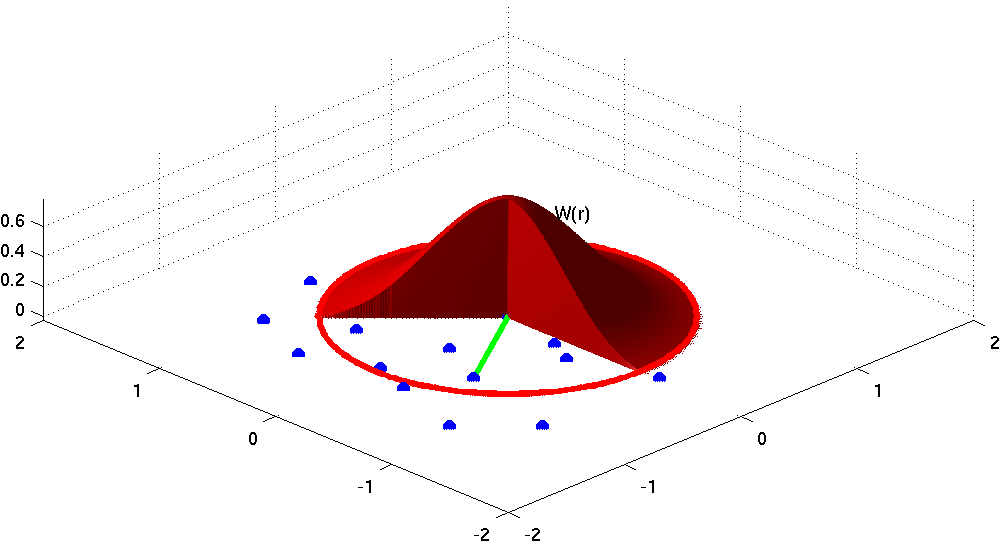
\includegraphics[angle=0,scale=0.4]{Figures/Apx_Topo/AGU_kernal.pdf}\\
\parbox{15cm}{\caption{\label{FigTopo_kernel}
Cubic spline smoothing interpolant.
}}
\end{figure}

The general equations for the cubic spline kernel are given below. For smoothing
the 2-D topographic data, we use $w_0=-\frac{10}{7\pi}$.

\begin{eqnarray*}
W(s) &=& \frac{w_0}{h^n} \left\{ \begin{array}
{l@{\quad:\quad}l}
1-\frac{3}{2}s^2+\frac{3}{4}s^3
& 0\le s<1 \\
\frac{1}{4}\left(2-s\right)^3
& 1\le s<2 \\
0 & s>1
\end{array}
\right.\nonumber \\
%\boldsymbol{\nabla} W(s) &=& \frac{w_0}{h^{n+1}} \left\{ \begin{array}
%{l@{\quad:\quad}l}
%-3s - \frac{1}{4}s^2 \,\boldsymbol{\hat{r}}
%& 0\le s<1 \\
%-\frac{3}{4}\left(2-s\right)^2 \,\boldsymbol{\hat{r}}
%& 1\le s<2 \\
%0 & s>2
%\end{array}
%\right.\nonumber \\
\end{eqnarray*}
\[
w_0=\frac{2}{3},-\frac{10}{7\pi} ,\frac{1}{\pi} \,\, \mathrm{for} \,\, \mathrm{1,2,3-D}
\]
Ash3d uses a value for $s$ provided as the `smoothing radius' in line 2 of the
topograpy block. If the value is much different than the grid spacing of the
meteorological files, a warning is issued.

Note, the smoothing approach outlined above is useful in mesh-free numerical
methods since gradients of functions can easily be expressed as a summation
of function values multiplied by the gradient of the kernel, however this can
lead to noisy gradient values when too few points contribute to the summation
or near boundaries. With the structured grid that Ash3d used, a finite difference
approach performs better.
%-> grad h with SPH vs FD
%(3) Interpolate to Met grid

\section{Numerical grid implementations}\label{ChapAppendTopo_Sec_GridImp}

\begin{figure}[htbp]\vspace*{0cm}\hspace*{0cm}
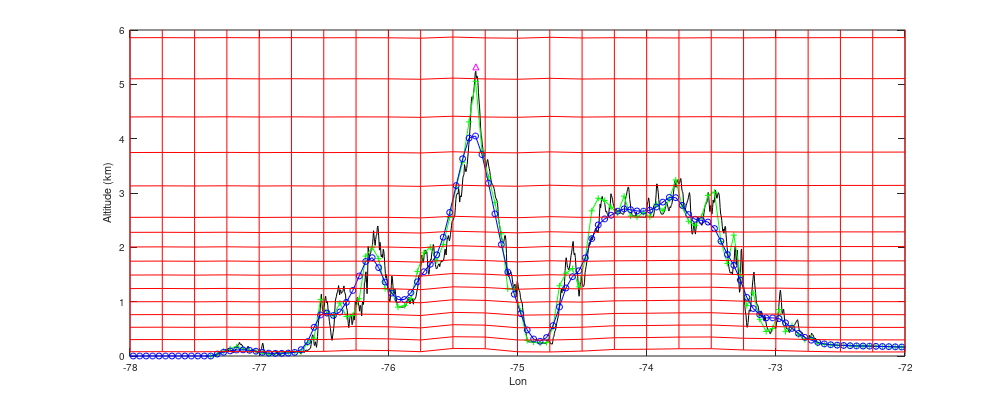
\includegraphics[angle=0,scale=0.4]{Figures/Apx_Topo/TopoRaw_Met.png}\\
\parbox{15cm}{\caption{\label{FigTopo_profile}
Transect of topography at a latitude of $4.895^{\circ}$ through Nevado del Ruiz.
GEBCO 2023 data is plotted with the black line. The sub-sampling of this topography
data onto the Ash3d computational grid is shown in green. Applying a 2-D smoothing filter
to the elevation data results in the blue line. The grid from the ERA5 NWP data is shown
in red with pressure levels plotted at the correspoding GPH values. The vent elevation
for Nevado del Ruiz is shown as a magenta triangle.
}}
\end{figure}



\begin{figure}[htbp]\vspace*{0cm}\hspace*{0cm}
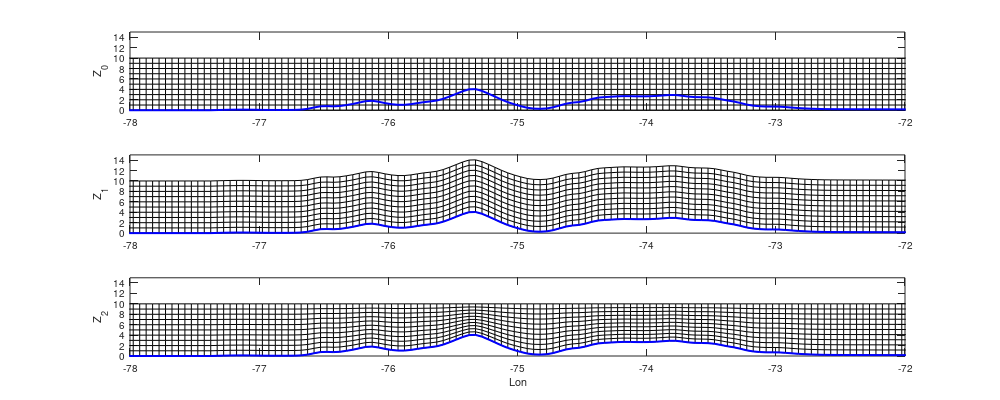
\includegraphics[angle=0,scale=0.4]{Figures/Apx_Topo/Topo_Grids.png}\\
\parbox{15cm}{\caption{\label{FigTopo_grids}
The standard vertical grid implementation in Ash3d is a uniform grid spacing from $z=0$
to $z=1.3*\mathrm{PlumeHeight}$, shown in the top plot. The smoothed topography from
Fig \ref{FigTopo_profile} is shown in blue. Implementing topography through a vertical
shifting of the grid is shown in the middle panel. Note that this grid extends above
$Z_{top}$ by the surface height. This sigma-altitude coordinate system is shown in the
bottom plot. This grid follows topography at the base, but tapers to a uniform upper-boundary
at $z=Z_{top}$.
}}
\end{figure}

\begin{figure}[htbp]\vspace*{0cm}\hspace*{0cm}
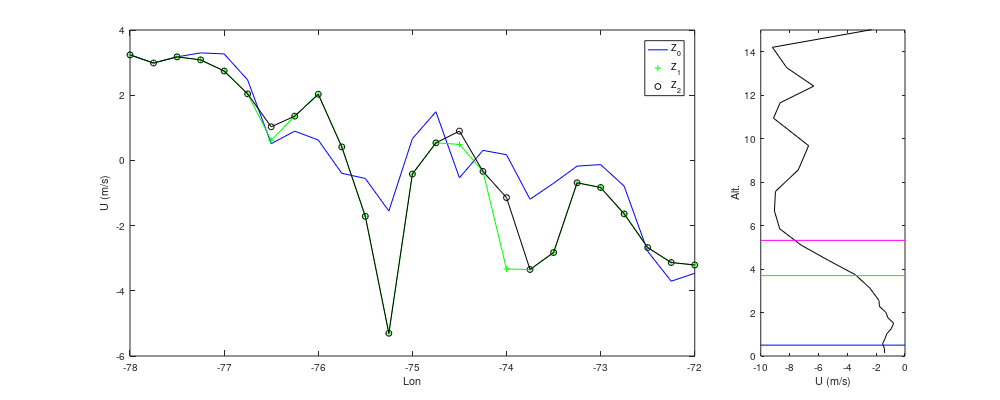
\includegraphics[angle=0,scale=0.4]{Figures/Apx_Topo/Topo_U.png}\\
\parbox{15cm}{\caption{\label{FigTopo_SurfU}
The three grids sample the NWP data at different heights
The case with no topography (1) samples pressure levels that are below topography
and are less reliable. The z-shifted grid case (2) samples values from the NWP file
at the appropriate pressure levels. The sigma-altitude coordinate system (case 3) also
samples values at the appropriate levels, but since it has thinner cells in regions with
high topography, the sample points are slightly different from the z-shifted
grid case. Plotted on the left are ERA5 zonal wind speeds ($U$) along the lowest grid
level for each of the three topography cases. On the right is a vertical profile plot of $U$
at the vent location showing where the lower level samples the NWP file for case 1 (blue),
2/3 (green) and at the vent elevation (magenta).
}}
\end{figure}

\subsection{Case 1: No deformation}
Recall that the governing advection-diffusion-sedimentation equation that Ash3d solves is
given by:
\begin{equation}\label{EqGovEqVectApx}
 \frac{\partial q}{\partial t} +
   \nabla \cdot \left[ \left(\mathbf{u} + \mathbf{v_s} \right) q \right]
 - \nabla \cdot \left( \mathbf{K} \nabla q\right) = S
\end{equation}
We will use a generanlized vertical coordinate, $X,Y,\sigma$, for all topography cases.
In the case of no grid deformation, this just corresponds to:
\begin{align*}
X &= x &  \frac{\partial}{\partial x} &= \frac{\partial}{\partial X}\\
Y &= y &  \frac{\partial}{\partial y} &= \frac{\partial}{\partial Y}\\
\sigma &= z &  \frac{\partial}{\partial z} &= \frac{\partial}{\partial \sigma}
\end{align*}
Obviously, the Jacobian of this `transformation' is: $J = |x_{i,j}| = 1$.

\subsection{Case 2: z-Shifted}
The z-shifted coordinate system is a simple shifting upward of the computational
grid with the topographic surface $h(x,y)$.
\begin{align*}
X &= x &  \frac{\partial}{\partial x} &= \frac{\partial}{\partial X}-\frac{\partial h}{\partial x}\frac{\partial}{\partial \sigma}\\
Y &= y &  \frac{\partial}{\partial y} &= \frac{\partial}{\partial Y}-\frac{\partial h}{\partial y}\frac{\partial}{\partial \sigma}\\
\sigma &= z-h(x,y) &  \frac{\partial}{\partial z} &= \frac{\partial}{\partial \sigma}
\end{align*}
In this case, the Jacobian remains $J = 1$.

Following the suggestions in \cite{Slordal02}, if we apply the substitution for the vertical
velocity in the transformed coordinate
\begin{equation}\label{v_sub1}
\omega = w - u \frac{\partial h}{\partial x} - v \frac{\partial h}{\partial y}
\end{equation}
and if we neglect topography terms of the diffusion term, then Eq. \ref{EqGovEqVectApx} can be
written in the transformed coordinates as:
\begin{equation}
\frac{\partial q}{\partial t} 
+ \frac{\partial }{\partial X} \left(uq\right)
+ \frac{\partial }{\partial Y}\left(vq\right)
+ \frac{\partial }{\partial \sigma}\left(\left( \omega + v_s \right) q\right)
- \frac{\partial}{\partial X} \left(K \frac{\partial q}{\partial X}\right) 
- \frac{\partial}{\partial Y} \left(K \frac{\partial q}{\partial Y}\right) 
- \frac{\partial}{\partial \sigma} \left(K \frac{\partial q}{\partial \sigma}\right) 
= S
\end{equation}
With this coordinate system, the same
fundamental equation can be used (Eq. \ref{EqGovEqVectApx}) with the implementation outlined
in Appendix \ref{ChapAppendFVSolvers}, simply with the substitution for vertical velocity given
by Eq. \ref{v_sub1}.

\subsection{Case 3: sigma-altitude}
An issue with the z-shifted coordinate system is that the effects of topography on the grid
are pervasive through $z$ and that the upper levels of the grid extend above the
set height of the domain, $Z_{top}$. An alternate systes in which the effects of
topograph decay with height is the sigma-altitude coordinate in which $Z_{top}$ is
fixed with $\sigma$-layers scaled into the space between $h(x,y)$ and $Z_{top}$.
\begin{align*}
X &= x &  \frac{\partial}{\partial x} &= \frac{\partial }{\partial X} + \frac{Z-\sigma}{D}\frac{\partial D}{\partial x}\frac{\partial }{\partial \sigma}\\
Y &= y &  \frac{\partial}{\partial y} &= \frac{\partial }{\partial Y} + \frac{Z-\sigma}{D}\frac{\partial D}{\partial y}\frac{\partial }{\partial \sigma}\\
\sigma &= Z \frac{z-h}{D} &  \frac{\partial}{\partial z} &= \frac{Z}{D} \frac{\partial}{\partial \sigma}
\end{align*}
where $Z=Z_{top}$ and $D(x,y)=Z-h(x,y)$, i.e. the depth of the computational grid at that $(x,y)$.
The Jacobian in this case is just $J=\frac{D}{Z}$.

This coordinate system is also outlined in \cite{Slordal02}, with a vertical velocity
substitution of
\begin{equation}\label{v_sub1}
\omega = \frac{Z}{D}w - \frac{Z-\sigma}{D}u \frac{\partial h}{\partial x} - \frac{Z-\sigma}{D} v \frac{\partial h}{\partial y}
\end{equation}
and, as in case 2, if we neglect topography terms of the diffusion term, then Eq. \ref{EqGovEqVectApx} can be
written in the transformed coordinates as:
\begin{eqnarray}
\frac{\partial q}{\partial t} 
&+& \frac{1}{D}\frac{\partial }{\partial X} \left(uDq\right)
+ \frac{1}{D}\frac{\partial }{\partial Y} \left(vDq\right)
+ \frac{1}{D}\frac{\partial }{\partial X} \left(\left( \omega + v_s \right)Dq\right) \\
&-& \frac{\partial }{\partial X} \left( K \frac{\partial q}{\partial X} \right) 
- \frac{\partial }{\partial Y} \left( K \frac{\partial q}{\partial Y} \right) 
- \left[\frac{Z}{D}\right]^2 \frac{\partial}{\partial \sigma} \left( K \frac{\partial q}{\partial \sigma} \right)
= S
\end{eqnarray}



%\subsection{Topography}\label{FV_Grid_Topo}
%https://nilu.brage.unit.no/nilu-xmlui/bitstream/handle/11250/2761899/08-2002-lhs.pdf
